\documentclass[a4paper]{article}
\usepackage[margin=3cm]{geometry}

\usepackage{graphicx}

\setlength{\parindent}{0cm}
\setlength{\parskip}{0.2cm}

\title{Trashootory\footnote{The name of the game is a hodgepodge of Trajectory, Shooting and Factory.} \\ An Exploration of Human's Innate Sense of Physics}
\author{Mathieu Triay \\ Cl\'ement Godard \\ Martijn van der Veen \\ Moos
Hueting}

\begin{document}

\maketitle

% Do we want a table of contents?
\tableofcontents
\pagebreak


% 2. Report:
% - One report per group should be given to us at the assessment time.
% - The report should present an overview of your project, including its aims and your approach.
% - Highlight any parts of the code or modeling that you are particularly proud of. In particular, highlight any interaction methods and ideas.
% - Include some screen captures.
% - Maximum of 5 pages.
% - PUT ALL GROUP MEMBER'S FULL NAMES ON THE REPORT!

% General introduction on assignment and CAVE
\section{Introduction}
Creating virtual environment applications is all about illusions. The better the
illusion, the better the user imagines to be in the virtual environment. A CAVE, 
with its immersive screens, tries to simulate the most important factor of illusion: 
vision. Combined with location tracking, physically realistic movements can be used 
in visually realistic applications.

In this report we present a new game created from scratch for the CAVE. In it, we experiment
with people's innate ability to work with physics. In the spirit of user experiences during
simulations, we will start off with the storyline of the game (section \ref{sec:story}),
followed by a more formal overview of the aim of the game in general and the aim of the
individual levels in particular (section \ref{sec:aim}). We will then lay out some
interesting elements in the specific approach (section \ref{sec:elements}), and end with
implementation details we think are noteworthy (section \ref{sec:inner}). As a conclusion, we'll discuss our journey with the CAVE and the improvements we had in mind for the game (section \ref{sec:discuss}).
% TODO: add conclusion? in that case, add one line here.


% Storyline, general approach
\section{The Story of the Game}
\label{sec:story}
You are subject to an experiment lead by university students which has the goal to, as they claim, 
``learn more about people's abilities to put in practice their innate sense of
physics''. The experiment says that you will have to throw things of different
weight and size at sometimes hidden targets and see how many tries it takes you
to get used to different objects and distances. The aim is to take down as many
targets as possible.

But as soon as you step in he experiment room, you notice something strange. The
room seems to be hanging above the ground and the lighting is very bad. You hear
strange sounds and suddenly you notice an odd blue light at your hand. The
atmosphere is clearly not a welcoming one anymore.

In front of you targets can be seen, which are badly hidden behind a stack of objects.
There are shelves on the walls in the experiment room, in which you find a wealth of
objects just as advertised by the experiment. When you pick up one of the objects,
the blue light disappears and you can't feel the weight of the object in your hand.
It seems like a large piece of wood.

When you try to drop it again, it unexpectedly hangs sinisterly in the air. Startled, you back
down and close your fist which has the effect of throwing the object into the big room
beyond the windows. You slowly start to realise that you can control the force of the
throw by moving your hand away from the object. The further you get, the further
it launches and its trajectory is determined by the position of your hand
compared to the position of the object.

After hitting all the targets the room seems to shake and suddenly moves upwards.
You see a new set of objects in front of your eyes with new targets in it. This
weird room hanging in the air is in fact an elevator and as you realise all this
you wonder how come you always find yourself in all sorts of dodgy experiments.

After you run out of objects to throw, the lift goes all the way up to the top of
the building where you find a sign telling you the experiment is over and that you
should quickly go back to your normal life.
% nice story ;-)


% Aims
\section{The Aim of the Game}
\label{sec:aim}

By using natural moving and a one-to-one mapping of real movements and events in
the game, the aim is to trigger, unconsciously, the inner physics calculation
abilities of the player. By using the experience learned while naturally throwing
or shooting objects in the real world, the user will slowly learn the variables
of the different aspects in the virtual environment he is standing in.

The game puts you in an uncomfortable situation (in a dark lift with odd sounds)
where you can lift any kind of object without being able to directly feel its weight,
and throw without on forehand knowing the effect of the `throwing vector'. This way
we want to make the player aware of, and let him use his, innate physics calculation
abilities.

Through trial and error he will slowly learn the weight of the different objects
and what distance is required to throw them at the force and trajectory he
wants. Also, he will be able to control in which way the objects are going by
moving his hand.

In everyday life you use your physics calculation abilities -- for instance when
you want to cross the road you are able to tell if a car is going to hit you or
not. In this case, however, most of the parameters are unknown. The player will
thus have to learn how to adjust himself to be able to complete the levels one
by one.

By recreating physics experiments with realistic body movement we hope to show the
player that he has unsuspected calculation skills and teach him how to use them
by going through different levels with various learning objectives.


% Levels (aims per level)
\subsection{Levels}
The user will have to complete five levels, each attempting to teach the user a
different aspect of the (natural) physics used in the game.

The first level has stacks of boxes quite near the lift and the goal is
visible just behind it. It is very likely that the player will shoot an object
right in front of him on the stack of cubes. If he shoots hard enough (the first
adjustment he must make), the scene cubes will fall on the goal, thus activating the lift.
He will get a basic idea about the correlation between throwing objects, and the
trajectory of the object outside the room he can't leave.

After this level, the basic workings of the levels should be fairly clear, but the
use and weight of all the objects as well as the precision of the trajectories is
still fairly poor.

The second level has stacks of boxes in the corner with goals behind. It is
supposed to teach the player how to adjust the direction of his object to hit the
stack of boxes hard enough and make the boxes fall on the goal.

In some cases, the boxes will fall but not on the goal so the user will have to
adjust the force they apply to the object for the second goal. Also, he will
have to aim accurately to shoot the goal located far away if the stacks failed
to trigger a domino effect causing the stacks to fall on the goal.

The targets of the third level are set in the air between walls. This is to
force the player to aim accurately and also encourage him to shoot from a
different vertical distance. In this case if the cube is set at waist height but
shot from a little under it should reach the goals. This is a relatively hard
level and it will take a lot of trial and error to get the trajectory right.

The fourth level has glass panes in front of the goals to try to teach you how
to use curved trajectories. It should teach you both how to aim vertically and
to control the throwing speed in order to make a certain trajectory.

The fifth level has a mix of all the different situation you encountered in
previous levels and should be considered as a sort of final examination telling
you if you managed to master your innate understanding of physics or not.


\section{Interesting Elements}
\label{sec:elements}
We will now discuss some less obvious, but interesting elements in the game.

\subsection{Elevator}

The elevator is essentially not part of the learning experience of the game.
We had to find a way of changing the levels without breaking the immersion.
The hard part of the CAVE experience is the fact that we cannot move beyond
the walls realistically, even though there might be a world out there.

Alternatives to the elevator were primarily vehicles like a car, a tank, a
plane or a helicopter. But for the game to be immersive in these moving confined places
without any real movement would be a hard challenge. Flying in a helicopter
where you cannot feel a thing is not exactly a thrilling experience.

The elevator fell more or less in this category but had two advantages over the
others. Firstly, the only movement occurs when the user doesn't interact with the
environment, and is only in the vertical direction (which humans are less used to).
Secondly, the sound of a lift is easily identifiable and can make you feel as if
you are moving relatively easy, furthermore we synchronised it with the elevator's
animation providing a greater immersive feeling. This is even more convincing with use of the 
wide-view visual feedback provided by the open windows. 

We also decided to make the ceiling
visible from the user in order to ensure that he feels inside the elevator and to avoid him 
trying to look above (since there is no screen).

You hear the sound and see everything around you move: it is just like you are taking
an elevator ride, with the CAVE being the elevator.

\subsection{Atmosphere}
The atmosphere of the game is slightly dark and can put you ill at ease at some
point. This was done partly to cope with the fact that you could not feel the objects
in your hand while throwing it and that you somehow use ``the force'' to throw them,
and to distract you from the impression that you should been familiarly with all the
aspect in this environment.\\
It is supposed to put you in a slightly recognisable place with familiar physics and
objects, but hint you at (and justify) your unusual and ``magical'' capabilities. The wand
controller has a physical power to lift objects without any effort and the unusual particle effect attached to
it is here to reinforce this feeling. Finally we added a light inside the hand controler
providing dynamic lighting following the movements of the hand to make the particle effect more realistic.


% Implementation
\section{Implementation Details}
\label{sec:inner}
For the game it was important that the trajectory and force of the launched objects was
more or less realistic, or at least with an equation which was sensible enough
to show quite major differences with not so major changes in hand position.

We have chosen to use a quadratic function for the speed, depending on the length
of the difference between the two clicks (times a constant that experimentally
turned out to be realistic). According to some sources
\footnote{http://www.wired.com/wiredscience/2010/10/physics-of-angry-birds/},
a quadratic function comes close to the actual physics behind a slingshot, which
has been the inspiration for the throwing/shooting interaction since most people
will be familiar with a slingshot. Our own trial and error have showed this quadratic
function to be reasonably realistic, apart from the fact that we don't also get
quadratic back pressure feedback while aiming.

Whilst programming the game we had to tweak Unity to do what we wanted it to do,
apart from the shooting physics, which resulted in a series of tricks which might
be worthy to talk about.
% TODO: talk about the lots of effort that was needed to also get it working i
%       the @#!!$$# CAVE?

The first trick is necessary to tell if a level is over or not. The number of goals to
hit per level is stored in a script called \verb!Win!, which should be attached to
all levels. \verb!Win! has a function named \verb!updateGoals! which should be called
every time a goal is hit and is in charge of decrementing the \verb!numberOfGoals! variable
When this variable reaches 0, we advance (activate the elevator to start moving) to the
next level.

All the goals in the level should have the \verb!Touch! script on them. This script calls
\verb!updateGoals! whenever it detects a collision and then disables itself.

This was the first use of the ``Script as objects'' feature of Unity. If you want
to use methods from another class, you have to include the script as a variable
that you initialise within Unity. This will let you access its methods and variables.

In this case, the \verb!Touch! script (on the targets) has the \verb!Win! script as a
variable and \verb!Win! has the \verb!Elevator! as a variable so it can play the key
frame animation defined on it.

Another interesting part of the inner workings is the way we track the number of
objects left to throw. Initially, for testing purposes, we stored this number in the
\verb!Catch! script, which was in charge of catching and shooting the object. When
we applied the force to the object to launch it, we also decreased the amount of
objects left.

But it turns out that as it is a variable which is needed by other parts of the
program (for example, to make the elevator move to the last level), so the script
has to be used as a variable by other scripts. The problem here was that the
\verb!Catch! script was written in C\# to be able to use the wand tracker, while
the other scripts were written in JavaScript. The mixing of the two did not work
well with Unity when it came to sharing scripts.

So instead, we created a new script (\verb!World!) which stores the number of levels
left to do and the number of objects left to throw and has two methods to update
these counters. The \verb!Update! function of this script checks if the number of
objects left to throw is greater than 0. If not, it means the game is over and you
go to the last level automatically. Furthermore, there is a loop which plays the
Elevator animation as many times as there are levels left to play.

To do all this, we had to find a way to update the number of objects.
However, we could not use the trick of the ``script as object'' in this case.
Instead we attached a new script (\verb!Thrown!) to the throwable objects which
checks if the state of the object is thrown or not. In this case, we set the
\verb!World! script as a variable of the \verb!Thrown! to keep track of them
globally. This way, we can also move the lift to the last level without problems.

\section{Conclusion \& Discussion}
\label{sec:discuss}
% TODO: write (very) short conclusion
%       (overal experience, things we didn't do but wanted to do)
In this project we have come up with a game in which the innate sense of physics
of people can be tested. Using multiple levels, each exploring a different aspect
of physics, the user is subjected to new situations in which haptic feedback is
not present. As such, the user learns the weights of the thrown objects and behaviour of the 
system by trial and error.

We have found by our own experience that through time one gets better at completing the levels.
A full user study to test the improvement over time would be a next step in the process.
From this user study we could also extrapolate the hardest part of the levels and see if
some of them are possibly too hard to hold the attention of the user.

Another improvement we have in mind is using the Kinect instead of the wand, to make the handling
of objects more natural. We envision a system where one hand holds the object and the other hand
acts as the force vector.

At the moment there is no haptic feedback at all. Some form of sense of touch would greatly increase
the power of the illusion. A study where we compare learning time between the system with and without
haptic feedback could yield interesting results.

Last but not least, the experience with working with the CAVE, although very exciting, has not always been a pleasant one.
A more robust system for working between the CAVE and our own personal computers would have
significantly improved our efficiency and would possibly have resulted in the inclusion of one or more of the above points.

\section{Game Visuals}

% TODO: add some nice screenshots and maybe photos of interaction in cave

%% image:

\begin{figure}[htbp]
	\centering
		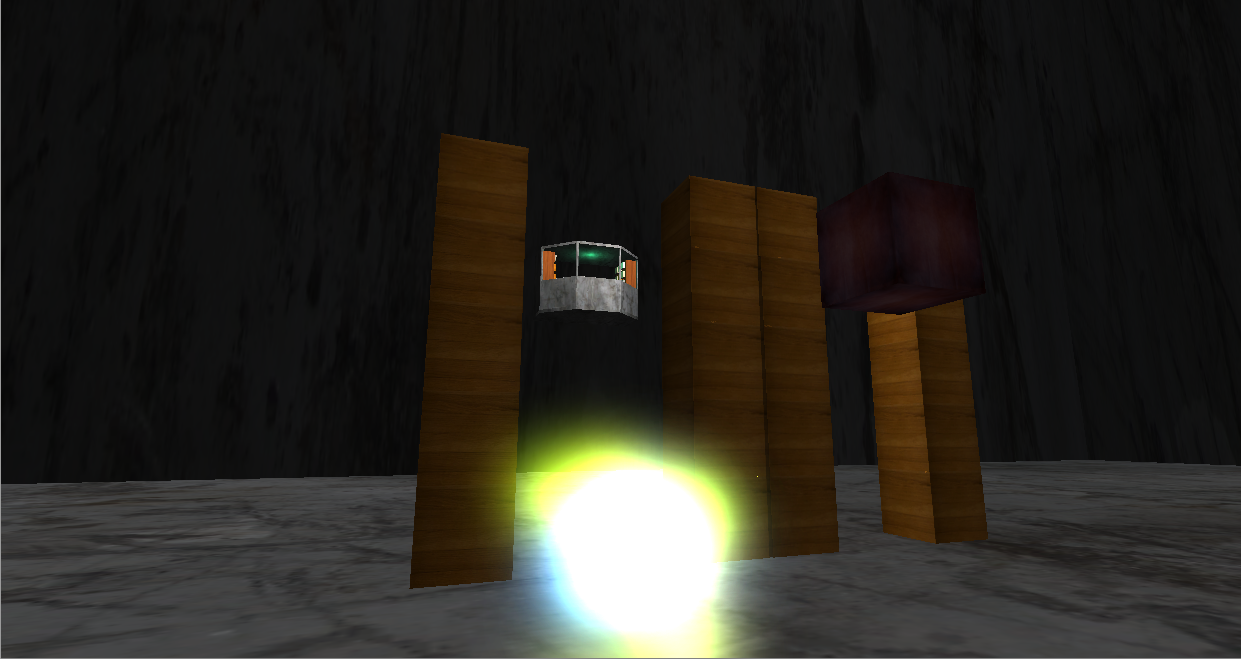
\includegraphics[width=1.0\textwidth]{level1-1.png}
	\caption{Level 1 - View from the level}
\end{figure}

\begin{figure}[htbp]
	\centering
		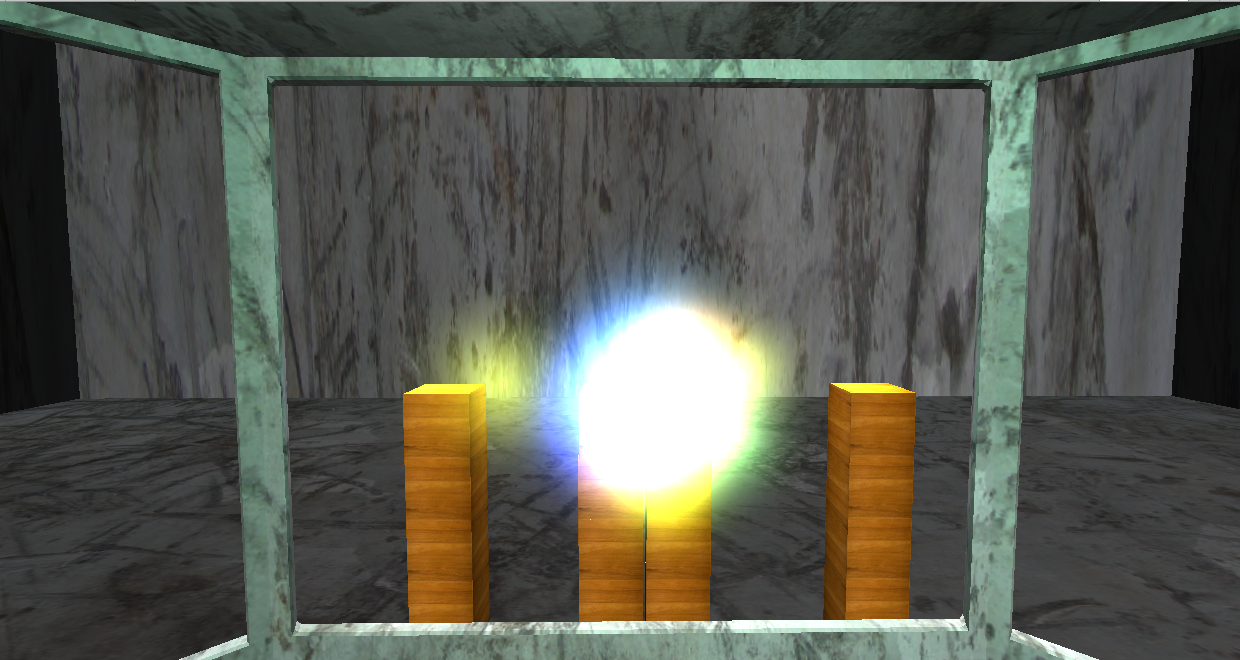
\includegraphics[width=1.0\textwidth]{level1-2.png}
	\caption{Level 1 - View from the elevator}
\end{figure}

\begin{figure}[htbp]
	\centering
		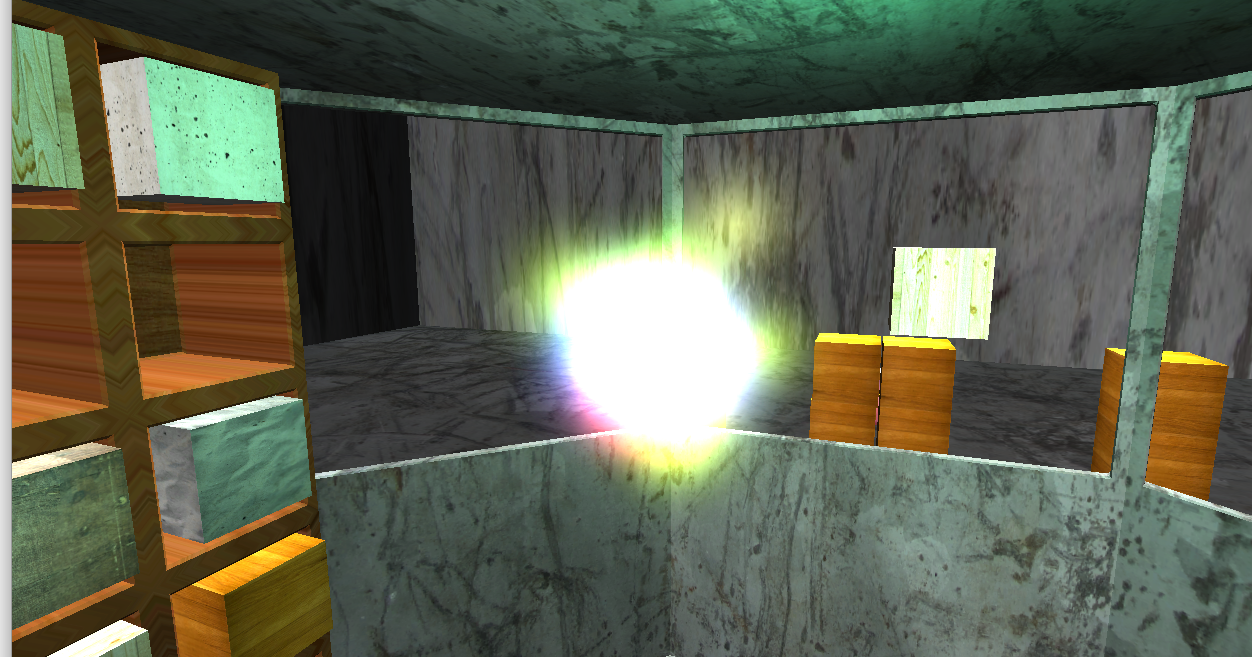
\includegraphics[width=1.0\textwidth]{level1-3.png}
	\caption{Level 1 - View with a box in the air}
\end{figure}

\begin{figure}[htbp]
	\centering
		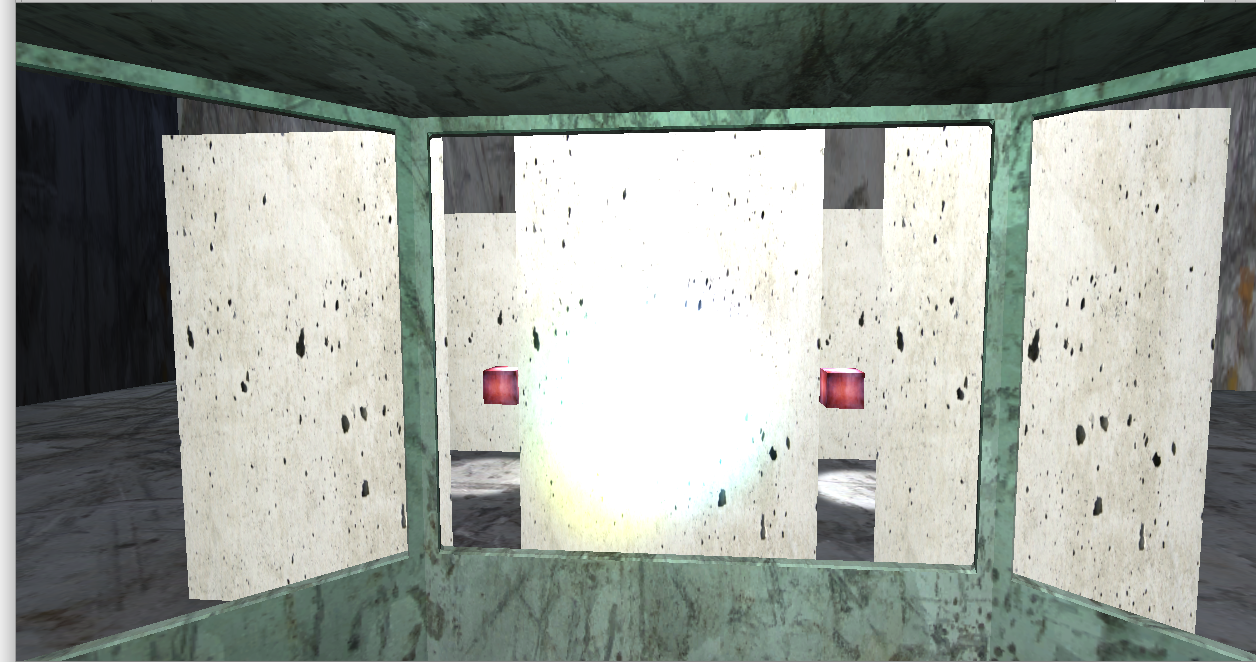
\includegraphics[width=1.0\textwidth]{level2.png}
	\caption{Level 2}
\end{figure}

\begin{figure}[htbp]
	\centering
		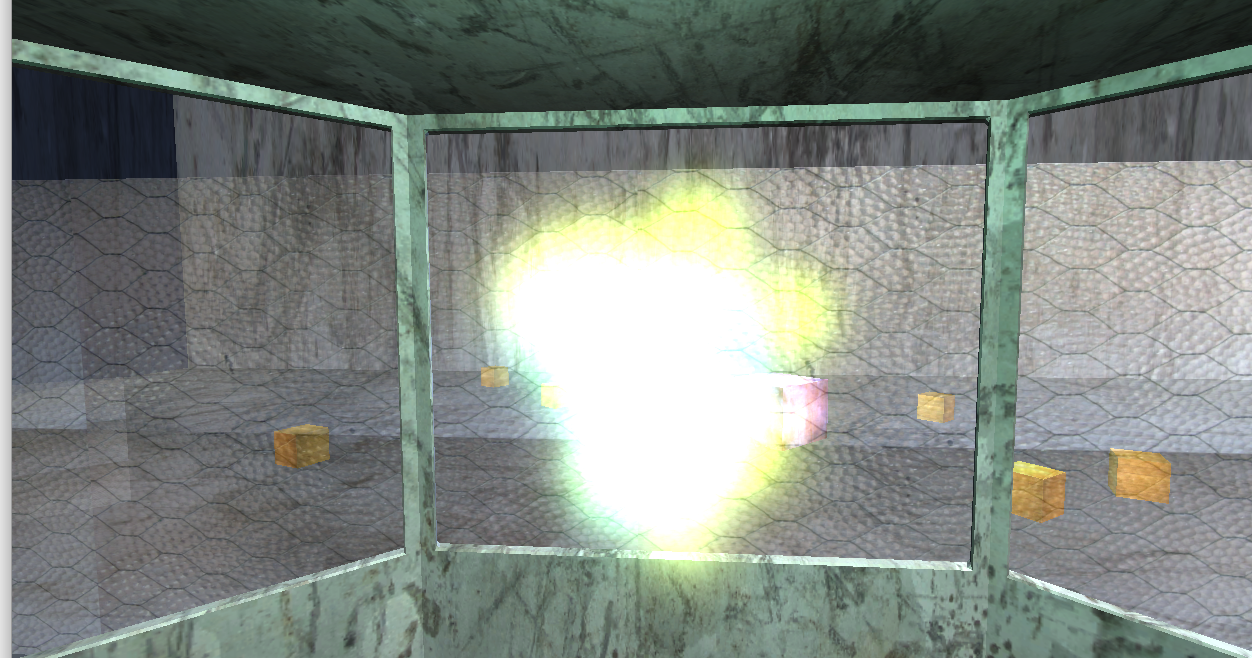
\includegraphics[width=1.0\textwidth]{level3.png}
	\caption{Level 3}
\end{figure}

\begin{figure}[htbp]
	\centering
		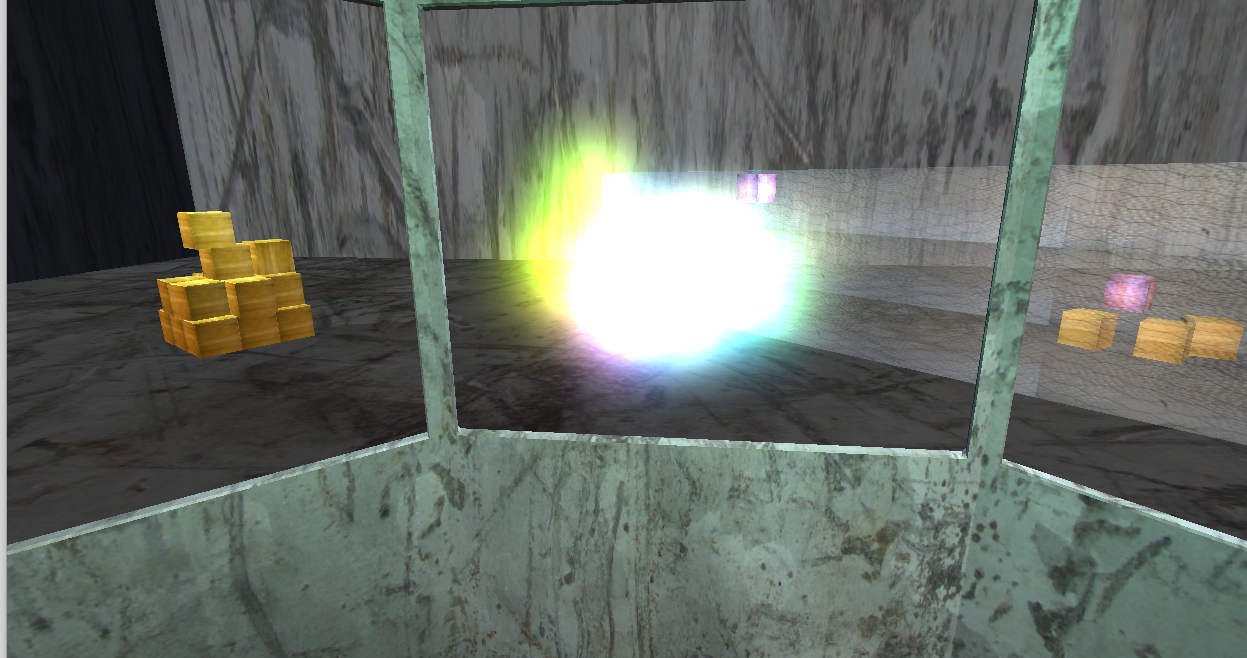
\includegraphics[width=1.0\textwidth]{level4.png}
	\caption{Level 4}
\end{figure}

\begin{figure}[htbp]
	\centering
		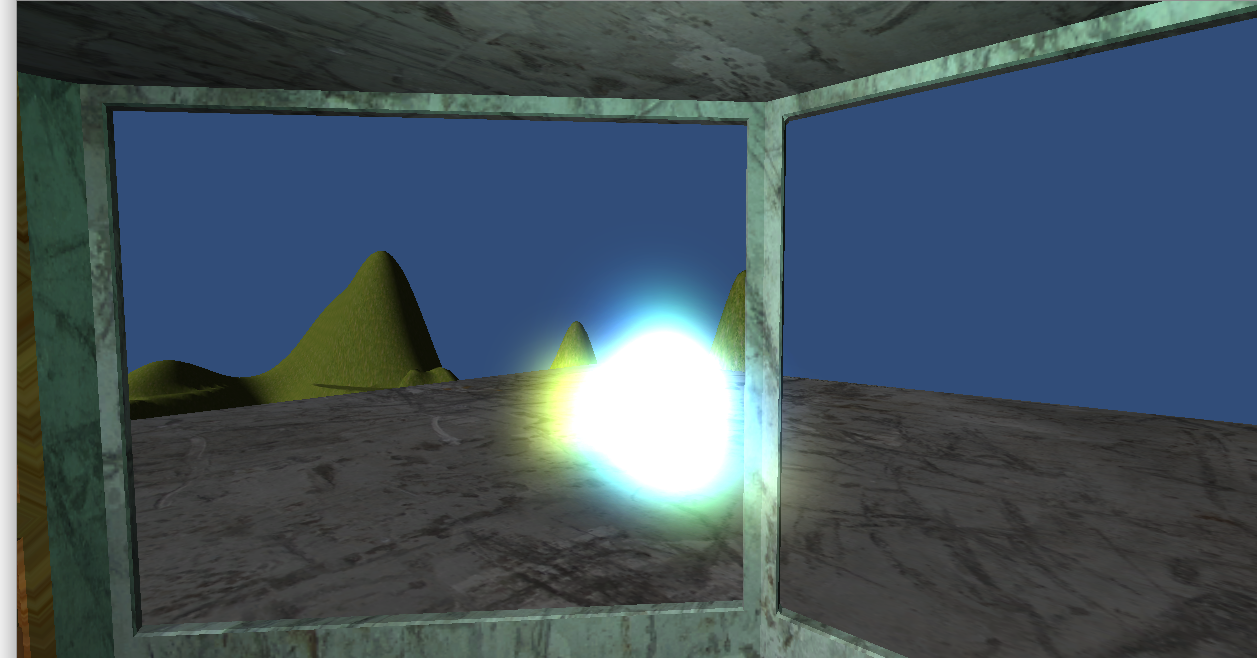
\includegraphics[width=1.0\textwidth]{end.png}
	\caption{The End}
\end{figure}

%% multi images:
%\begin{figure}[ht]
% \centering
% \subfigure[]{
%  \includegraphics[width=1.0\textwidth]{img/}
%  \label{fig:}
% }
% \subfigure[]{
%  \includegraphics[width=1.0\textwidth]{img/}
%  \label{fig:}
% }
% \caption{}
% \label{fig:}
%\end{figure}


% TODO: now drink some beer


\end{document}
